\chapter{仕事とエネルギー}

{\small 注: この章を理解するには, 数学リメディアル教材で「積分」を理解していることが必要。}

本章では「エネルギー」について学ぶ。世の中には「エネルギー」という言葉が溢れているが, 
なぜそんなに「エネルギー」って大事なのだろうか? ていうか, そもそも「エネルギー」って
何なのだろうか? それを理解するには, まず「仕事」という概念を定義しなければならない。
そこから話をはじめよう。\\

\section{仮想仕事の原理}

前章で, 体を滑車に吊るす話や, 動滑車で物を持ち上げる話や, 質量の異なる物体を
2つの斜面に置いてロープでつないで静止させる話などを学んで, 君は不思議に
思わなかっただろうか? これらの話は, とりあえず力のつりあいや, 作用・反作用
の法則などは, 満足させている。だが, 物体をその重さの半分の力で
持ち上げられる, というのは不思議だ。我々の日常感覚では, ある物を持ち
上げるにはその重さと同じ力が必要では? と, シンプルに考えてしまう。
しかし実際の自然はそうではない。不思議だ。気持ち悪い。この不思議さ
をうまく説明し, この気持ち悪さから我々を救ってくれるシンプルな法則
は無いのだろうか? 

それが, ここで学ぶ「仮想仕事の原理」だ。これは「力のつりあい」
を, もっと普遍的に述べた物理法則である。「力のつりあい」と等価だが, ある意味, それ
よりも深く, 根源的なものを内包した法則だ。

\begin{exmpl}
動滑車で物を持ち上げる話(問\ref{q:force_rope4})では, 滑車やロープや天井などが
互いに及ぼす力(張力など)は別とすれば, 関与する力は, 君がロープを下向きに引く力$T$と, 物体に
下向きにかかる重力$mg$だ。ここで, 仮想的に, 君がロープを, ちょっとだけ引っぱった
としよう(図\ref{fig:string4vw})。このとき, 滑車Bが$\Delta x$だけ持ち上がったとする。
すると, 当然, 物体も同じだけ, つまり$\Delta x$だけ持ち上がる。このとき, ロープの動きを
たどって考えれば, 君がロープを引っ張った長さは$2\Delta x$であることがわかるだろう
\footnote{滑車Bの左右端からそれぞれ長さ$\Delta x$だけ上の部分が, 
引っ張った後には無くなっている。これらの長さの合計は(左右にそれぞれ1つずつあるので)
$2\Delta x$である。}。
\begin{figure}[h]
    \centering
    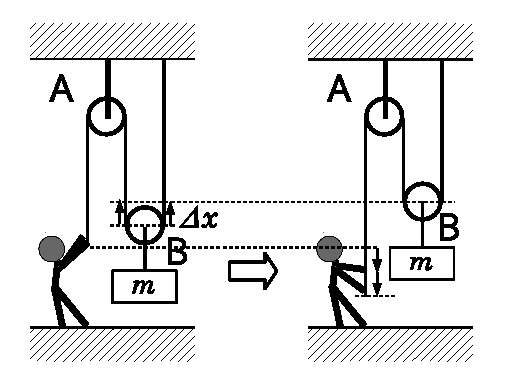
\includegraphics[width=8cm]{string4vw.eps}
    \caption{動滑車を使う持ち上げ。物体を$\Delta x$だけ上昇させるには
ロープを$2\Delta x$だけひっぱる必要がある。}\label{fig:string4vw}
\end{figure}

このとき, 下向きに座標をとり, それぞれの力と, その力が働く点が動いた距離の
掛け算を考え, それを合計してみる。
\begin{eqnarray}
T(2\Delta x) + mg (-\Delta x)
\end{eqnarray}
ここで, 第二項の$(-\Delta x)$のマイナスは, 座標の向き(下向き)とは
逆の上向きに物体が移動することをあらわす。で, \underline{\textgt{だまされたと思って, 
これを0とおいてみよう}}:
\begin{eqnarray}
2T\Delta x - mg \Delta x=0
\end{eqnarray}
すると, 
\begin{eqnarray}
T=\frac{mg}{2}
\end{eqnarray}
という, 正しい答えが得られる。これが仮想仕事の原理の例である。(例おわり)
\end{exmpl}

仮想仕事の原理とは以下のようなものである:
\begin{itembox}{仮想仕事の原理}\index{かそうしごとのげんり@仮想仕事の原理}
力がつりあっている系では, 仮想的な微小変位に伴って外力のなす仕事の総和は0である。
\end{itembox}

「仮想的な微小変位」とは, 上の例で言えば, 君がロープを引く
$2\Delta x$や, 物体が上に上がる$\Delta x$のことだ。
「外力」とは, 君が引く力と, 物体にかかる重力のことだ。
そして, 
\begin{itembox}{仕事の定義}\index{しごと@仕事}
「力と, その力が働く点が"力と同じ向き"に動いた距離との掛け算」を「\underline{仕事} (work)」という。
\end{itembox}

なんで「仕事」とか「仮想的な微小変位」とかの得体の知れぬものを持ち出してこんな
「原理」を考えるのだろうか? それは, こうすればうまく(シンプルに無矛盾に)
いろんな物事を説明できるからだ。なぜこんな原理が成り立つのか, その
理由は誰も知らない。自然はそうなっているのだ。

この例では, 確かに動滑車のおかげで, ロープを引っ張る力は半分になったが, 
そのかわり, ひっぱる長さは倍になってしまった。つまり, 同じ高さだけ持ち上げ
ようとすると, かかる力が半分なら, ひっぱる長さ(距離)を倍にしなければならない。
つまり, たとえ必要な力は動滑車などで変えることができても, 力と距離の掛け算, 
つまり仕事は, 変えることができない。それが自然の摂理なのだ。だから, 
仕事という概念が便利なのだ。

もうひとつの例を考えよう。前章で考えた, 2つの斜面に物体を置いてロープで
つないで静止させる話である。
\begin{figure}[h]
    \centering
    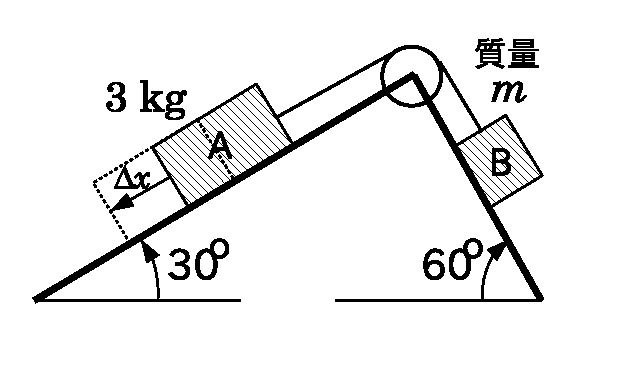
\includegraphics[width=7cm]{slope4b.eps}
    \caption{2つの斜面に載せられ, ロープでつながって静止する2つの物体。図\ref{fig:slope4}改変。}\label{fig:slope4b}
\end{figure}
\begin{exmpl}
前章の問\ref{q:force_rope2}において, 物体Aを斜面に沿って
左下向きに$\Delta x$だけ動かしてみよう(図\ref{fig:slope4b})。すると, ロープにつながっている物体Bも, 
斜面に沿って左上向きに$\Delta x$だけ動くはずだ。このとき, 
物体Aに関して重力がなす仕事は, (3~kg)$g\{\sin(\pi/6)\}\Delta x$である。一方, 
物体Bに関して重力がなす仕事は, $-mg\{\sin(\pi/3)\}\Delta x$である。マイナスがつくのは, 物体Bが重力
と逆方向(上方向)に移動したからだ。仮想仕事の原理より, 
\begin{eqnarray}
\Bigl(3\text{ kg})g\Bigl(\sin\frac{\pi}{6}\Bigr)\Delta x-mg\Bigl(\sin\frac{\pi}{3}\Bigr)\Delta x=0
\end{eqnarray}
ここから, $m=\sqrt{3}$~kgが出てくる。(例おわり)
\end{exmpl}

%
\begin{q}\label{q:def_work} 
\begin{enumerate}
\item 仕事とは何か?
\item 仕事の単位をSI基本単位による組み立て単位で表せ。それをJ(ジュール)と呼ぶ。
\item 仮想仕事の原理とは何か? 
\end{enumerate}
\end{q}
\mv

%
\begin{q}\label{q:teko}
君は「てこの原理」\index{てこのげんり@てこの原理}を聞いたことがあるだろう。これは仮想仕事の
原理から導くことができる。図\ref{fig:balance}上のように, 支点Sの上に, 
左右に長さ$l_1$, $l_2$を持つ「てこ」が置かれ, 左右それぞれの端にぞれぞれ質量
$m_1$, $m_2$の物体1, 2が載っている。これを, 図\ref{fig:balance}下のように, 
左側が下がるように, 仮想的に小さな角$\theta$だけ下げる。このとき, 
\begin{enumerate}
\item 左端がもとの状態から$h_1$だけ下がり, 右端がもとの状態より$h_2$だけ上がるとすると, 
\begin{eqnarray}
h_1&=&l_1\sin\theta \\
h_2&=&l_2\sin\theta
\end{eqnarray}
となることを示せ。
\item 物体1における重力による仮想仕事は$m_1gl_1\sin\theta$, 
物体2における重力による仮想仕事は$-m_2gl_2\sin\theta$となることを
示せ。 
\item 仮想仕事の原理より, 次式(てこの原理)を導け:
\begin{eqnarray}
m_1l_1=m_2l_2\label{eq:principle_balance}
\end{eqnarray}
\end{enumerate}
\end{q}
\begin{figure}[h]
    \centering
    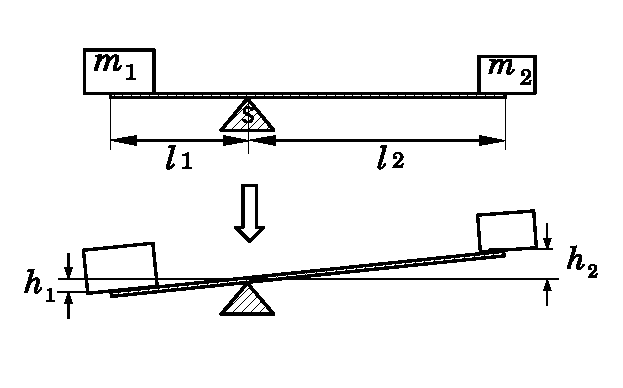
\includegraphics[width=7cm]{balance.eps}
    \caption{仮想仕事の原理からてこの原理を導く。}\label{fig:balance}
\end{figure}

前章で述べたように, 物体が静止しているとき, 「力のつりあい」が実現している。
しかし, 実は, 「大きさを持つ物体」についてはそれに加えて, 上述の「てこの原理」
に相当する, 「モーメントのつりあい」\index{もーめんとのつりあい@モーメントのつりあい}
というものも実現する。モーメントとは, 簡略に言えば, ある点(支点)からの距離と, 
それに直交する力との積だ。そして, モーメントのつりあいとは, モーメントの
合計が0になるということだ。高校物理を学んだ人は聞いたことがあるだろう。
しかし, これをきちんと正しく記述し, 理解するには, 数学で「ベクトルの外積」
というのを学ばねばならないので, 今は詳述しない(後の章で学ぶ)。ただし, 
ここでは, 「仮想仕事の原理は, 力のつりあいだけでなく, モーメントのつりあいまでも
含んだ, 一般性の高い法則だ」ということを認識しておこう。\mv

\begin{q}\label{q:jack}
図\ref{fig:jack}のようなジャッキについて, 半径$r$のハンドルを1回転すると, 
上載物は$\Delta y$だけ持ちあがるとする。摩擦は無視する。
\begin{enumerate}
\item ハンドルをまわすのに必要な力を$F$とする。ハンドルを1回転するときに, 君の手がなす仕事は
\begin{eqnarray}2\pi r F\end{eqnarray}
であることを示せ。
\item 上載物の質量を$m$とする。ハンドルを1回転するときに, 重力のなす仕事は
\begin{eqnarray}-mg\Delta y\end{eqnarray}
であることを示せ。
\item 次式を示せ:
\begin{eqnarray}2\pi r F-mg\Delta y=0\end{eqnarray}
\item 次式を示せ:
\begin{eqnarray}F=\frac{mg\Delta y}{2\pi r}\end{eqnarray}
\item $m=1000$~kg, $r=0.2$~m, $\Delta y=0.003$~mのとき, $F$はどのくらいか?
\end{enumerate}
\begin{figure}[h]
    \centering
    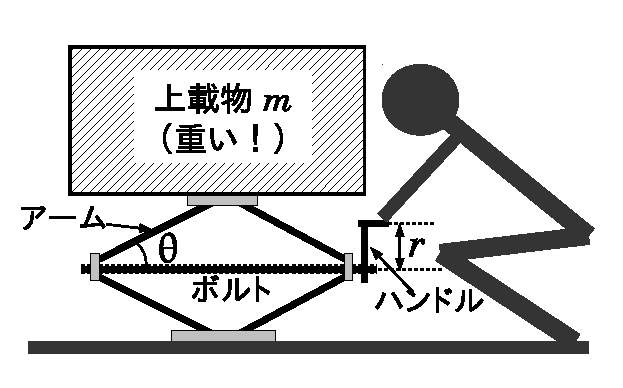
\includegraphics[width=6cm]{jack.eps}
    \caption{ジャッキで物を持ち上げる。}\label{fig:jack}
\end{figure}
\end{q}

\begin{faq}{\small\textgt{仮想仕事の原理の「仮想的な微小変位」
はどうして仮想的である必要があるんですか?}
... 「微小変位」という考え方自体がそもそも仮想的です。バランスしている系に
少しでも変化を加えたら, バランスが崩れるかもしれない。でも, 「バランスを崩さない程度に
小さな変位」というのが微小変位であって, そもそもそんなの厳密には
現実的に無理じゃね?という気持ちがあるから「仮想」なのです。}\end{faq}\mv

\begin{faq}{\small\textgt{仮想仕事の原理に鳥肌が立ちました。
自然の不思議さを感じざるを得ません。}
... このような原理を見つける旅が, 学問としての物理学なのでしょう。}\end{faq}
\hv



\section{仕事とエネルギー}

さて, 仮想仕事の原理では, 「仕事」という量が重要な働きをした。それにとどまらず, 
仕事は, 物理学の全般にわたって, 重要な役割を果たす概念だ。例として, 
図\ref{fig:string4vw}の例をもういちど考えよう。君がロープを引くことで
\begin{eqnarray*}2T\Delta x\end{eqnarray*}
という仕事をしたとき, 同時に, 質量$m$の物体にかかる重力が
\begin{eqnarray}-mg\Delta x\end{eqnarray}
という仕事をした。このとき, 仮想仕事の原理から, 両者の和は0である。

君がロープを引くことによって君は仕事をし, 実際, 疲れる。しかしその努力は, 
重力に逆らって物体が上昇した, という結果(重力による負の仕事)に残っている。
この上昇した状態で物体に別のロープとか滑車とかてこをつければ, 今度は物体が
下がることによって, また別の物体を持ち上げることができるだろう。

このような話は, お金のやりとりに似ていないだろうか? A君がB君に1000円を譲渡したとする。
なぜそんなやりとりが起きたか, とか, それによって2人の関係はどうなるか, という興味も
あるが, 2人以外の人にしてみれば, お金のやりとりは2人の間で完結している(2人あわせた
収支は0である)。そして, A君からもらった1000円で, こんどはB君がCさんから
何かを買うことができる。

物理学における仕事とは, この話の「お金」のような役割をする。A君, B君, Cさん, ...
とお金が手渡されていくように, 君がロープを引くことでなした仕事は, 後々まで, 形を変えながら, 
様々なところに受け渡されるのだ。そのように, 仕事を普遍化した
量を, 物理学では\underline{エネルギー}\index{えねるぎー@エネルギー}という。
\textgt{エネルギーとは, 仕事が形を変えた量, もしくは仕事に形を変えることができる量である}。
エネルギーは仕事と同じ次元を持ち, その単位は, SI単位系ではJである。

\begin{q}\label{q:energy}
エネルギーとは何か? 
\end{q}

エネルギーには, 様々な形態がある。熱もエネルギーだ。
なぜか? 例えば気体に熱を加えると膨張し, まわりのものを移動
させることができる。つまり, 仕事ができる。だから熱はエネルギーである。

光もエネルギーの一形態だ。なぜか? 太陽光を浴びると暖かくなる, 
つまり熱を受け取ることができる。熱はエネルギーなので, 光はエネルギー
を運ぶのだ。

熱は, 後に学ぶ「運動エネルギー」というタイプのエネルギーに
帰着させて考えることができる。また, この章の後半で学ぶ
「ポテンシャルエネルギー」というタイプのエネルギーもある。
物質が化学反応するときに出る熱や光は, 物質の分子レベルでの
ポテンシャルエネルギーの変化によるものである。\mv

さて, 仕事について, もう少し, 丁寧に数学的に意味づけよう。

さきほど, 仕事とは, 「力と, その力が働く点が"力と同じ向き"に動いた距離との掛け算」である
と述べたが, それが成立するのは, その点の移動中に, 力がほとんど変化しないことが
必要である(でなければ, どの時点での力を掛け算すればいいのかわからない)。では, 
移動中に力が次第に変化するような場合は, 仕事はどのように定義されるのだろうか? 

%2011.4.2 ヤマサキ 仕事の定義を定式化する中の, シグマをインテグラルにするところ。今のリメディアルの記述と整合的にするために式を追加。
いま, ある物体に力$F$がかかっているとき, それを力の向きに$\Delta x$だけ
動かす。 $\Delta x$だけ動かす間には$F$は変化しないと考える。すると, その力がする仕事$\Delta W$は, 
\begin{eqnarray}
\Delta W=F\Delta x \label{eq:work}
\end{eqnarray}
である。これは仕事の定義だ。これをたくさん繰り返すことを考えよう。
いま, 座標上で, 位置$x_0$にある物体を, 位置$x_1$まで運ぶとする。
この間, 物体にかかる力は変化するかもしれないが, $x_0$から$x_1$
まではとても近くて, その間の力の変化は無視できるくらいに小さいと
する(逆に言えば, 力の変化が無視できるくらいに, $x_0$と$x_1$を
近づける)。つまり, この間の力は$F_1$でほぼ一定値とみなせる。このときの
仕事$\Delta W_1$は, 上の式から, 
\begin{eqnarray}\Delta W_1\fallingdotseq F_1\Delta x_1\end{eqnarray}
である($\Delta x_1=x_1-x_0$とする)。位置$x_1$まで来た物体は, 
こんどは$x_1$のすぐ近くの位置$x_2$まで運ばれ, その間, 物体にかかる力は$F_2$で一定で
あるとする(ただし$F_2$は$F_1$と同じとは限らない)。このとき
の仕事$\Delta W_2$は, 同様に, 
\begin{eqnarray}\Delta W_2\fallingdotseq F_2\Delta x_2\end{eqnarray}
である($\Delta x_2=x_2-x_1$とする)。以下同様に, 物体
をすこしずつ$x_3, x_4, \cdots, x_n$まで順次運び($n$は正の整数), 各
ステップでは物体に$F_3, F_4, \cdots, F_n$というそれぞれ一定値の
力がかかっていると, 各ステップでの仕事は, 
\begin{eqnarray}
\Delta W_3\fallingdotseq F_3\Delta x_3\nonumber\\
\Delta W_4\fallingdotseq F_4\Delta x_4\nonumber\\
\cdots\nonumber\\
\Delta W_n\fallingdotseq F_n\Delta x_n\label{eq:W_nF_nDx_n}
\end{eqnarray}
となる。これらを辺々で合計すれば, 
\begin{eqnarray}\sum_{k=1}^{n}\Delta W_k\fallingdotseq \sum_{k=1}^{n}F_k\Delta x_k\end{eqnarray}
となる。左辺は, 物体を$x_0$から$x_n$まで運ぶときの全体の仕事であり, これを
$W$と書こう:
\begin{eqnarray}
W\fallingdotseq \sum_{k=1}^{n}\Delta W_k\fallingdotseq\sum_{k=1}^{n}F_k\Delta x_k \label{eq:one_step_before_work2}
\end{eqnarray}
ここで$n$を十分大きくとって, $x_1, x_2, ..., x_n$の分割を十分に細かく
すれば, すなわち, \eref{eq:one_step_before_work2}の極限として, 
\begin{eqnarray}
W=\lim_{\substack{n\rightarrow \infty\\\Delta x_k\rightarrow 0}}\sum_{k=1}^{n}F_k\Delta x_k
\end{eqnarray}
を考えれば, 「数学リメディアル教材」の積分の定義より, 次式が成り立つ:
\begin{itembox}{仕事の定義(力が一定でない場合)}
物体を位置$a$から位置$b$まで運ぶときの仕事は, 
\begin{eqnarray}
W=\int_{a}^{b} F(x)\,dx \label{eq:work2}
\end{eqnarray}
\end{itembox}
ここで$x_0$を$a$に, $x_n$を$b$に, 改めて書き換えた。$F(x)$は$x$の各点で物体が受ける力
だ。この式(\ref{eq:work2})は, 仕事の定義式(\ref{eq:work})を, 「力が次第に
変化する場合」に拡張した(つまり, より一般性の高い)仕事の定義式である。\mv

\begin{exmpl}\label{ex:work_fall}
 質量$m$の物体が, 地表付近で$mg$という大きさの重力を受けて, 高さ$h_0$から$h_1$まで
変化する。重力のなす仕事を求めよう。座標軸を上向きにとると, 重力は, 式(\ref{eq:gravity_earth})より, 
\begin{eqnarray}F=-mg\end{eqnarray}
である。ここで右辺のマイナスは, 重力が座標軸の向きとは逆向きであることを表す
\footnote{式(\ref{eq:gravity_earth})では力の向きを考えず, 力の大きさだけを考えていたことに注意せよ。}。
従って, 式(\ref{eq:work2})より, 
\begin{eqnarray}
W&=&\int_{h_0}^{h_1} (-mg)\,dx\nonumber\\
 &=&-mg(h_1-h_0)=mg(h_0-h_1)
\end{eqnarray}
となる。もし$h_0>h_1$なら(つまり物体が下がるとき), $W>0$である。
もし$h_0<h_1$なら(つまり物体が上がるとき), $W<0$である。つまり, 重力に
逆らって動く場合は, 重力のする仕事はマイナスである, ということになる。(例おわり)
\end{exmpl}

\begin{faq}{\small\textgt{例\ref{ex:work_fall}で, 座標軸は下向きじゃダメですか?}
... いいですよ。その場合, $F=mg$となり, $W=mg(h_1-h_0)$。これは本文の結果とは符号が
逆のように見えますが, 今の場合は$h$が大きいと低いので, 結局, 物体が下がると$h_0<h_1$となり, 
そのとき$W$は正になる。 という結論は変わりません。本文で座標を上向きにとったのは, 
「高いところほど$h$が大きい」ほうが, 我々の空間認識では直感に素直だからです。}\end{faq}
\mv

\begin{exmpl}
質量$m$の物体Aが, 質量$M$の物体Bから万有引力を受けながら, 物体Bからの
距離が$R_0$から$R_1$まで変化する。このとき万有引力のなす仕事を求めよう。座標軸を
物体Bから物体Aの向きにとると, 万有引力は, 式(\ref{eq:gravity_univ})より, 
\begin{eqnarray}F=-\frac{GMm}{x^2}\end{eqnarray}
である。ここで右辺のマイナスは, 万有引力が座標軸の向きとは逆向きであることを表す
\footnote{式(\ref{eq:gravity_univ})では力の向きを考えず, 力の大きさだけ
を考えていたことに注意せよ。}。式(\ref{eq:work2})より, 
\begin{eqnarray}
W&=&\int_{R_0}^{R_1} \Bigl(-\frac{GMm}{x^2}\Bigr)\,dx=\Bigl[\frac{GMm}{x}\Bigr]_{R_0}^{R_1}\nonumber\\
 &=&GMm\Bigl(\frac{1}{R_1}-\frac{1}{R_0}\Bigr)\label{eq:work_gravity}
\end{eqnarray}
となる。(例おわり)
\end{exmpl}
\mv

%
\begin{q}\label{q:spring_work}
バネ定数$k$のバネについた物体を, バネの自然状態を原点として位置$x_0$
から位置$x_1$まで動かすときに, バネの弾性力がなす仕事$W$は, 
\begin{eqnarray}
W=-\frac{1}{2}\,k\,(x_1^2-x_0^2)\label{eq:spring_work}
\end{eqnarray}
となることを示せ。ヒント: 式(\ref{eq:Hooke})より$F=-kx$とし, 式(\ref{eq:work2})を使う。
\end{q}
\vspace{0.2cm}

%
\begin{q}\label{q:gas_work}
気体を膨張させたり圧縮したりするときの仕事を考えよう。ある気体が, 断面積$A$の
シリンダー(筒状の容器)に入っており, 上面がピストンで蓋してある。
鉛直上向きに$x$軸をとり, シリンダーの底面で$x=0$とする。ピストンは$x$軸にそって上下に
動くことができる。最初, ピストン(つまり蓋)は$x=h$にあって静止しているとする
(図\ref{fig:gas_piston})。
ピストンは十分に軽いとし, 重力を無視する。気体の圧力を$P$とする。
\begin{figure}[h]
    \centering
    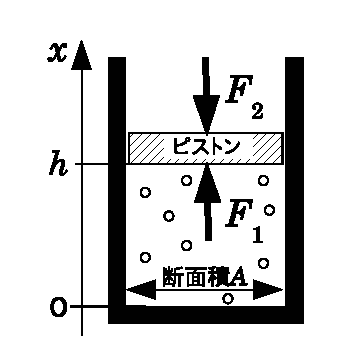
\includegraphics[width=7cm]{gas_piston.eps}
    \caption{気体の入ったシリンダー。}\label{fig:gas_piston}
\end{figure}
\begin{enumerate}
\item 気体の体積$V$は, $V=Ah$と表せることを示せ。
\item 気体がピストンに及ぼす力$F_1$は, 
\begin{eqnarray}F_1=PA\label{eq:gas_work1}\end{eqnarray}
となることを示せ。
\item 外部からピストンにかかる力(それを外力という\footnote{この外力が
具体的に何によるものかは, ケースバイケースであり, ある場合は誰かが手で押さえ
込んでいるのかもしれないし, ある場合はシリンダー外部に充満する気体
の圧力によるものかもしれない。この問題ではその詳細は気にしない。})
を$F_2$とすると, 
\begin{eqnarray}F_2=-PA\label{eq:gas_work2}\end{eqnarray}
となることを示せ。
\item 次に, ピストンをゆっくり動かして, $x=h+dh$の位置に移動させることを考えよう。
$dh>0$なら, 気体は膨張し, $dh<0$なら気体は圧縮される。$dh$は微小であり, 
ピストンが$x=h$から$x=h+dh$まで動く間に$F_1$や$F_2$はほとんど一定である
とみなす。このとき, 外力がなす仕事$dW$は, 
\begin{eqnarray}dW=F_2\,dh=-PA\,dh\label{eq:gas_work3}\end{eqnarray}
となることを示せ。
\item 体積の変化を$dV$とする。すなわち, ピストンの移動後に気体の体積は
$V+dV$になったとする。次式を示せ:
\begin{eqnarray}dV=A\,dh\label{eq:gas_work4}\end{eqnarray}
\item \eref{eq:gas_work3}, \eref{eq:gas_work4}より次式を示せ:
\begin{eqnarray}dW=-P\,dV\label{eq:gas_work5}\end{eqnarray}
\item ピストンを大きく動かし, 体積が$V_1$から$V_2$になるまで変化させることを考えよう。
この間に外力がなす仕事$W$は次式のようになることを示せ:
\begin{eqnarray}
W=-\int_{V_1}^{V_2}P\,dV
\end{eqnarray}
\item ここで, 気体は理想気体であるとしよう。つまり, 理想気体の状態方程式:
\begin{eqnarray}PV=nRT\end{eqnarray}
が成り立つとする($n$はモル数, $R$は気体定数, $T$は絶対温度)。次式が成り立つことを示せ:
\begin{eqnarray}
W=-\int_{V_1}^{V_2}\frac{nRT}{V}\,dV
\end{eqnarray}
\item ここでさらに, ピストンの移動は十分にゆっくりであり, その過程では温度$T$は
一定であるとすると, 次式が成り立つことを示せ:
\begin{eqnarray}
W=nRT\ln\frac{V_1}{V_2}
\end{eqnarray}
\item 1モルの理想気体を摂氏0度(一定)で体積を半分まで圧縮するときに外力がなす仕事を求めよ。
\end{enumerate}
\end{q}
\vspace{0.2cm}

\eref{eq:gas_work5}は, 化学や熱力学で, 非常によく出てくる式だ。ここでは外力が
なす仕事を考えたが, 気体(の圧力)がなす仕事を考えると, それは外力がなす仕事の符号を
逆にしたものである(なぜなら気体がピストンにおよぼす力は外力がピストンにおよぼす
力の逆だから)。それを$dW'$とすると, $dW'=-dW$なので, 
\begin{eqnarray}
dW'=P\,dV
\end{eqnarray}
となる。この式もよく使われるので, \eref{eq:gas_work5}との違いをよく理解して
おこう\footnote{化学や熱力学では, 教科書によって, 外力のなす仕事を$dW$とするものと, 
気体がなす仕事(すなわちここで$dW'$とあらわしたもの)を$dW$とするものがあるので, 
気をつけよう。}。
\hv


\section{ポテンシャルエネルギー}\index{ぽてんしゃるえねるぎー@ポテンシャルエネルギー}

さて, \eref{eq:work2}をみると, 仕事$W$は, 始点$a$と終点$b$の関数だ。特に, 始点$a$
をどこかに固定して(それを基準点と呼ぼう), $W$を$b$だけの関数とみなし, 改めて$b$を$x$と
書けば, $W$は$x$の関数$W(x)$だ。その意味は, 「基準点から位置$x$まで物体を
運ぶときの仕事」である。この$W(x)$の符号を変えたものを\underline{ポテンシャルエネルギー}
\footnote{「位置エネルギー」とか, 単に「ポテンシャル」と言うこともある。}という。すなわち, 
\begin{itembox}{ポテンシャルエネルギーの定義(1)}
\begin{eqnarray}
U(x)=-W(x)\label{eq:potential}
\end{eqnarray}
で定義される関数$U(x)$を, 「\textgt{ポテンシャルエネルギー}」という。
ここで$W(x)$は, 物体を基準点から位置$x$まで運ぶときに, 物体にかかっている力がなす仕事である。
\end{itembox}

\begin{exmpl}\label{ex:gravity_potential_mgh}
上の例\ref{ex:work_fall}で, 地面を基準点とすれば, $h_0=0$となり, $h_1$を
改めて$h$とおけば, $W(h)=-mgh$である。このとき, ポテンシャルエネルギーは, 
\eref{eq:potential}から, 
\begin{eqnarray}
U(h)=mgh\label{eq:potential_g}
\end{eqnarray}
である。(例おわり)
\end{exmpl}

つまり, 物体を高く持ち上げるほど, 重力によるポテンシャルエネルギーは, 
大きくなる。で, 持ち上げられた物体は, てこや滑車を使えば, 別の物体を持ち上げる「仕事」を
することができる。つまり, ポテンシャルエネルギーとは, 力を受けている物体が, ある位置に
あることによって持つエネルギー, つまり位置に付随するエネルギーである。


%
\begin{q}\label{q:def_potential}
ポテンシャルエネルギーとは何か? 
\end{q}

ところで, \eref{eq:potential}の右辺の$W(x)$は, 物体にかかっている力
がなす仕事だ。例えば例\ref{ex:gravity_potential_mgh}では, 重力がなす仕事がそれに相当する。
ところが, 現実的には, 重力がかかっている物体が, ひとりでに重力に逆らって上に移動したりは
しない。誰かが重力に逆らう力をかけて, その物体を持ち上げねば, 物体は上に移動しない。
そのような「誰かの力」がなす仕事$W'(x)$を考えると\footnote{ここで$W'(x)$のダッシュ
は「微分」という意味ではない。単に$W(x)$と区別するための印である。}, それは重力
のなす仕事とは同じ大きさでありながら符号が逆である(力の向きが逆だから)。
すなわち, $W'(x)=-W(x)$だ。それを使うと, ポテンシャルエネルギーは以下のように
定義することもできる:

\begin{itembox}{ポテンシャルエネルギーの定義(2)}
\begin{eqnarray}
U(x)=W'(x)\label{eq:potential2}
\end{eqnarray}
で定義される関数$U(x)$を, 「\textgt{ポテンシャルエネルギー}」という。
ここで$W'(x)$は, 物体を基準点から位置$x$まで運ぶときに, かかっている力に逆らって
誰かがなす仕事である。
\end{itembox}

例\ref{ex:gravity_potential_mgh}では, 物体を地面から高さ$h$まで君が持ち上げる
とすれば, 君は物体に上向きに$mg$という大きさの力をかけ, 上向きに$h$だけ移動
させねばならないので, そのとき君がなす仕事は$W'(h)=mgh$だ。従って
ポテンシャルエネルギーは, \eref{eq:potential2}から, $U(h)=mgh$となり, 
それは\eref{eq:potential_g}に一致する(つじつまが合っている)。

\eref{eq:potential}と\eref{eq:potential2}は, 互いに等価であり, どちらの
定義を採用してもかまわない。これらの2つの定義は, 教育的な意味で, 「わかりやすさ」
に一長一短があるのだ。前者は, 右辺にマイナスが出てくるのがちょっと不自然で
わかりにくい。後者は, そこに実在している力とは別の力を誰かが発揮すると想定する
という点でわかりにくい。そこで, これらの欠点を解消した第3の定義がある。すなわち, 

\begin{itembox}{ポテンシャルエネルギーの定義(3)}
\begin{eqnarray}
U(x)=W''(x)\label{eq:potential3}
\end{eqnarray}
で定義される関数$U(x)$を, 「\textgt{ポテンシャルエネルギー}」という。
ここで$W''(x)$は, 物体を位置$x$から基準点まで運ぶときに, 物体にかかっている力
がなす仕事である。
\end{itembox}

例\ref{ex:gravity_potential_mgh}で, 物体が高さ$h$から地面(基準点)まで落下する
ことを考えれば, 下向きに$mg$という大きさの重力がかかって, 下向きに$h$だけ移動
するので, そのとき重力がなす仕事は$W''(h)=mgh$である。従って
ポテンシャルエネルギーは, \eref{eq:potential3}から, $U(h)=mgh$となり, 
それは\eref{eq:potential_g}に一致する(つじつまが合っている)。

もちろん, \eref{eq:potential}, \eref{eq:potential2}, \eref{eq:potential3}
は, 互いに等価であり, どれを定義として採用してもかまわない(ちょっと考えれば, 
$W''(x)=W'(x)=-W(x)$であることがわかるだろう)。教科書や学者によって, どの定義を
採用するかは, 様々だ。しかし, 物理学の実体としては, どれも同じことだ。\mv

\begin{q}\label{q:potential_spring}
バネ定数$k$のバネについた物体を考える。バネの自然状態を原点かつ基準点として, 
物体が位置$x$にあるとき, バネの弾性力によるポテンシャルエネルギー$U(x)$は次式の
ようになることを示せ。また, 関数$U(x)$をグラフに描け。
\begin{eqnarray}
U(x)=\frac{1}{2}kx^2\label{eq:potential_spring}
\end{eqnarray}
\end{q}
\mv

\begin{q}\label{q:potential_gravity}
質量$m$の物体が, 質量$M$の物体から距離$R$だけ離れているときの, 万有引力に
よるポテンシャルエネルギー$U(R)$を考える。無限遠($R=\infty$)を基準点とすると, 
$U(R)$は次式のようになることを示せ。また, 関数$U(R)$をグラフに描け。
\begin{eqnarray}
U(R)=-\frac{GMm}{R}\label{eq:potential_gravity}
\end{eqnarray}
\end{q}
\mv

実は, \eref{eq:potential_gravity}は, \eref{eq:potential_g}を一般化した式である。
前者から後者を導出できるのだ。やってみよう。今, 地球の質量を$M$, 地球の半径を$R_0$, 
地表からの高さを$h$とすると, 地表から高さ$h$にある, 質量$m$の物体のポテンシャル
エネルギーは, \eref{eq:potential_gravity}より, 
\begin{eqnarray}
U(R_0+h)&=&-\frac{GMm}{R_0+h}
=-\frac{GMm}{R_0}\frac{R_0}{R_0+h}\nonumber\\
&=&-\frac{GMm}{R_0}\frac{1}{1+h/R_0}
\end{eqnarray}
となる。ここで, $h<<R_0$, すなわち, 高さは地球の半径に比べて十分に小さいとすると, 
\begin{eqnarray}
\frac{1}{1+h/R_0}\fallingdotseq 1-\frac{h}{R_0}
\end{eqnarray}
である。これを上の式に代入すれば, 
\begin{eqnarray}
U(R_0+h)&\fallingdotseq&-\frac{GMm}{R_0}\Bigl(1-\frac{h}{R_0}\Bigr)\nonumber\\
&=&-\frac{GMm}{R_0}+\frac{GMmh}{R_0^2}\label{eq:pot_grav_approx_08}
\end{eqnarray}
となる。ここで, 地表での重力を考えれば, 
\begin{eqnarray}
\frac{GMm}{R_0^2}=mg
\end{eqnarray}
である。これを使って\eref{eq:pot_grav_approx_08}を書き換えると, 
\begin{eqnarray}
U(R_0+h)\fallingdotseq-\frac{GMm}{R_0}+mgh\label{eq:pot_grav_approx_09}
\end{eqnarray}
となる。ここで, 
\begin{eqnarray}
U(R_0+h)+\frac{GMm}{R_0}
\end{eqnarray}
を$U(h)$と書き換えれば(これは基準点を地表面に変更することに相当する), \eref{eq:potential_g}を得る。\\

\begin{q}\label{q:potential_etc}
以下の値をそれぞれ求めよ。必要な数値は, 各自, 調べよ。
\begin{enumerate}
\item 地上10~mの高さにある, 質量2~kgの物体に関する, 重力のポテンシャルエネルギー。
\item 長さ10~m, 直径2~mmの鉄線を1~mm伸ばしたとき, 鉄線の弾性力のポテンシャルエネルギー。
\item 月に関する, 地球の重力のポテンシャルエネルギー。
\end{enumerate}
\end{q}
\mv

\begin{q}\label{q:slope_lift_energy1}
傾斜角$\theta$の滑らかな斜面に沿って, 質量$m$の物体を, 斜距離$L$だけ運びあげた。かかった仕事は? 
また, ポテンシャルエネルギーの変化は? 
\end{q}
\mv

ここでひとつ注意。ポテンシャルエネルギーという考え方は, 物体にかかる力が
\underline{保存力} (conservative force)\index{ほぞんりょく@保存力}
という, ある種の力についてのみ, 成り立つ。
保存力とは, 物体を移動させるとき, その力がなす仕事が, 移動の経路
によらず, 出発点と到達点だけで決まる, というような力である。

そもそも, ポテンシャルエネルギー$U(x)$とは, ある特定の位置(基準点)から位置$x$まで
物体を運ぶときに力がなす仕事を用いて定義された。力が保存力
でなければ, この$W(x)$が移動の経路によってまちまちの値をとりうるので, $W(x)$の
値が$x$で一意的に定まらない。つまり, $U(x)$の値が一意的に定まらないのだ。

我々が考えうる力の多くは保存力である。数少ない例外は, 摩擦力だ。摩擦力は保存力ではない。
\mv

%
\begin{q}\label{q:conservative_force}
保存力とは何か? 
\end{q}
\mv

\begin{q}\label{q:NewtonLaw_mistake} 上の問について, 以下のような
回答があった。それぞれについて, 正しいか, 正しくないか, 正しくないならどこがどのように
間違っているかを述べよ。
\begin{enumerate}
\item 「物体を移動させるとき, どの経路をたどっても仕事が変わらないもの」
\item 「物体を移動させるとき, その力がなす仕事が, 移動の経路
によらず, 出発点と到達点だけで決まること」
\item 「物体を移動させるとき, その力がなす仕事が, 移動の経路
によらず一定であるような力」
\item 「物体を移動させるとき, 移動の経路によらず一定であるような力」
\end{enumerate}
\end{q}
%答まだ。


%
\begin{q}\label{q:friction_non_conservative}
摩擦力が保存力でないことを証明しよう。
\begin{enumerate}
\item 物体を位置$x_0$から位置$x_1$に運ぶときの仕事を$W_{01}$とし, その逆戻り, つまり
物体を位置$x_1$から位置$x_0$に運ぶときの仕事を$W_{10}$とする。もし力が保存力なら, 
$0=W_{01}+W_{10}$
となることを示せ(ヒント:物体を$x_0$から$x_0$まで運ぶ経路には, 「何も動かさない」とか
「$x_0$から$x_1$までを往復する」などがある。)
\item 摩擦力では, 上の式が成り立たないことを示せ。
\end{enumerate}
\end{q}
\mv

\begin{q}\label{q:slope_lift_energy2}
傾斜角$\theta$の, 動摩擦係数$\mu'$の斜面に沿って, 質量$m$の物体を, 
斜距離$L$だけ運びあげた。かかった仕事は? また, 重力のポテンシャルエネルギーの変化は? 
\end{q}
\hv


\section{仕事率}
単位時間あたりになされる仕事のことを, \underline{仕事率}\index{しごとりつ@仕事率}と
いう。すなわち, 時間$\Delta t$の間に, 仕事$\Delta W$が行われた場合, 仕事率$P$は, 
\begin{eqnarray}P = \frac{\Delta W}{\Delta t}\label{eq:work_rate0}\end{eqnarray}
と定義される。ここで, 仕事率が時々刻々と変わるような場合についても
対応できるように, $\Delta t$として十分に短い時間をとると, 
\begin{eqnarray}P = \frac{dW}{dt}\end{eqnarray}
となる。つまり, 仕事率は, 仕事を時刻で微分したものである, と言ってもよい。\mv

\begin{exmpl}
質量$m$の物体を, $\Delta t$の時間をかけて高さ$\Delta h$まで持ち上げる
場合を考えよう。仕事$\Delta W$は$mg\Delta h$となる。仕事率$P$は, 
\begin{eqnarray}P= \frac{\Delta W}{\Delta t}= \frac{mg \Delta h}{\Delta t}\end{eqnarray}
となる。$\Delta t$を0に近づけると, 
\begin{eqnarray}P= mg\frac{dh}{dt}\end{eqnarray}
となる。$dh/dt$は物体を持ち上げる速度だ。これを$v$とおくと, 
\begin{eqnarray}P= mgv\label{eq:work_rate_lift}\end{eqnarray}
となる。(例おわり)
\end{exmpl}

数学リメディアル教材で学んだように, 仕事率の単位は, SI単位系で表すと, 
kg~m$^2$ s$^{-3}$, もしくは, 同じことだがJ s$^{-1}$だ。この単位を
ワットといい, Wとあらわす。\mv

\begin{q}\label{q:work_rate}
質量2.0~kgの物体を, 地表付近で, 3.0~m/sの速さで持ち上げる時の仕事率を求めよ。
\end{q}

\eref{eq:work_rate0}を見ると, ぶっちゃけ言えば仕事率は「仕事を時間でわったもの」
であることがわかる。この関係を逆転すると, 仕事率に時間をかけたら仕事になる, 
ということがわかる\footnote{正確には, 仕事率を時刻で積分したものが仕事になる。}。
なので, 仕事の単位として, 「仕事率かける時間」という単位を使うこともできる。
特によくあるのが, 仕事率をW, 時間をhで表す, W~h (ワット時)という単位だ。
これは仕事の単位, すなわちエネルギーの単位だ。1~Wの仕事率を1~時間続けたとき
の仕事が, 1~W~hだ。

\begin{q}\label{q:watt_hour}
1~W~hのエネルギーを, Jを単位として書きなおせ。
\end{q}
\hv



\section{電位・電位差・電圧}

小中学校理科で, よく「電圧」とか「ボルト」というのが出てきた。
しかし実は, 電圧の定義は, 小学生や中学生が理解できるような
ものではないのだ。あのときは電圧は「水路の高さ」とか
「その差」とかいう喩え話で教えられたが, ここで本当の定義を
君に教えよう。その前に以下の問題をやって欲しい:

\begin{q}\label{q:potential_Coulomb}
原点に電荷$Q$を持つ物体1があり, 位置$x$に, 電荷$q$を持つ物体2が
あるときの, クーロン力によるポテンシャルエネルギー$U(x)$は次式になることを示せ:
\begin{eqnarray}
U(x)=\frac{k\,Q\,q}{x}\label{eq:potential_Coulomb}
\end{eqnarray}
ただし, 無限遠を基準点とする。$k$は\eref{eq:coulomb}に現れる定数である。
\end{q}
\mv

前問のように, 電気的な力 (クーロン力) によるポテンシャルエネルギーは, 
電荷に比例する。そこで, 電気的なポテンシャルエネルギーについては, 
それをその場所の電荷で割った値で表現することが多い。
それを\underline{電位}\index{でんい@電位}と呼ぶ。つまり, 電位とは
「その場所の単位電荷あたりのポテンシャルエネルギー」と定義するのだ。

電位の単位は, SI単位系では J~C$^{-1}$である。これをVと書き, 「ボルト」と呼ぶ。

空間の2点の間の, 電位の差を\underline{電位差}\index{でんいさ@電位差}
という。電位差のSI単位は電位と同じくVである。

\begin{q}\label{q:potential_Coulomb2} 問\ref{q:potential_Coulomb}の
続き。
\begin{enumerate}
\item 物体1が位置$x$に作る電位を式であらわせ。
\item 100年ほど前の理論(ボーアの原子模型という)では, 
水素原子は, 陽子から0.529$\times10^{-10}$~mの
付近に電子があると考えられていた。その付近の電位は何Vか?
\end{enumerate}
\end{q}

空間の2つの点の間を仮想的に荷電粒子を移動させるとき, 
かかる仕事を電荷で割ったもの(単位電荷あたりの仕事)
を, その2点間の\underline{電圧}\index{でんあつ@電圧}
とか\underline{起電力}\index{きでんりょく@起電力}
という(定義)。電圧や起電力のSI単位もVである。

多くの場合, 電位差と電圧(起電力)は同じだ。ただし, 
電位差と電圧が異なることもある。それは, 電気的な力がクーロン力だけでなく, 
磁場の時間的変化によってももたらされる場合である。
その場合は, 電気的な力は保存力ではなくなる(経路によって
仕事が変わる)。その詳細については, 君の現在の数学力では理解
できないので, 本書では述べない。とりあえず, そういう場合は, 
電位差よりも電圧や起電力という言葉が用いられる, ということを頭の
片隅に置いておこう。

\begin{q}\label{q:potential_Volt} 
\begin{enumerate}
\item 電位とは何か?
\item 電圧とは何か?
\item 電位の単位をSI単位系で述べよ。
\item 2~Vの電位に0.3 Cの電荷があるときのポテンシャルエネルギーを求めよ。
\item 1~Vの電位に電子が1個あるときのポテンシャルエネルギーを求めよ。
\end{enumerate}
\end{q}
\mv

問\ref{q:potential_Volt}(5)で考えた, 1~Vの電位にある電子1個の
ポテンシャルエネルギーの絶対値である
$1.602\times10^{-19}$~Jは, 1~eVと呼ばれる。\underline{eV}\index{eV}は
\underline{エレクトロン・ボルト}\index{えれくとろんぼると@エレクトロン・ボルト}という
新たな単位であり, 電子や原子や分子の様々な形のエネルギーを表現する
のによく使う。特に化学でよく使う。\mv

\begin{q}\label{q:radiation_eV} 原子核崩壊で出る放射線に, 
$\alpha$線, $\beta$線, $\gamma$線というのがある。
$\alpha$線はヘリウム原子核が飛んでくるもの, $\beta$線は電子が飛んでくるもの, 
そして$\gamma$線は光の一種(ただしとても波長が短い)だ。ヘリウム原子核の
質量を$m_{\text{He}}$とし, 電子の質量を$m_{\text{e}}$とする。
\begin{enumerate}
\item $m_{\text{He}}$を求めよ。ヒント: Heの質量数は4。つまり1~molのHeの質量は4~g
だ。He原子核はHe原子よりも, 電子2個ぶん軽いが, その差は無視してよい。
\item 放射性元素プルトニウム239の崩壊で発する$\alpha$線のエネルギーは, 
$\alpha$粒子1個あたり5.5~MeVである。このときの$\alpha$粒子の速さを求めよ。
\item 放射性元素セシウム137の崩壊で発する$\beta$線のエネルギーは, 
電子1個あたり510~keVである。このときの電子の速さを求めよ。なお
$m_{\text{e}}$=9.1$\times10^{-31}$~kgである。
\end{enumerate}
ヒント: ここでいう「エネルギー」は運動エネルギーである。
\end{q}
\hv




\section{電流・電力・電力量}

\pref{sect:CoulombForce}で, 電荷とは何かを学んだ。
ここでは「電流」を学ぼう。導線の中などで, ある場所を
多くの荷電粒子が次々と通り過ぎるとき, 通り過ぎた荷電粒子の電荷の総量を, 
それにかかった時間でわったものを\underline{電流}\index{でんりゅう@電流}
という(定義)。すなわち, 単位時間あたりに通り過ぎる電荷
が電流である。

定義から, 電流は, C/s (クーロン毎秒)という単位で
表現できることがわかる。C/sという単位をA (アンペア)と
いう\footnote{AはSI基本単位
のひとつなので, 本来はC=A~sがCの定義なのだが, 君は
A=C/sがAの定義だと思っておくほうがわかりやすいだろう。}。\mv

電気的な力によって行われる仕事の仕事率 (単位時間あたりの仕事)
を\underline{電力}\index{でんりょく@電力}という(定義)。
特に, 電圧$V$の2点間を電流$I$が流れている
ときの仕事率は$VI$となる。なぜか? 電荷$q$が電圧$V$の2点
間を移動するときの仕事は$qV$である(それが電圧の定義!)。
それを時間$\Delta t$で行ったなら, 仕事率は$qV/\Delta t$
だ。ところが, $q/\Delta t$は, 移動した電荷を時間で
割ったものだから, それは電流$I$である。従って, 仕事率は$VI$。

$V$の単位はV, つまりJ/Cであり, $I$の単位はAだから, 
$VI$の単位はJ~A/Cである(ここで出てきた, 斜字体の$V$と立体の
Vは, 互いに意味が違うことに君は気づいているだろうか? 
数学リメディアル教材で学んだように, 斜字体は変数, 立体は
単位を表す約束だった!)。ここで, C=A~sであることを思い出すと, 
J~A/Cは結局, J/s, つまりW (ワット)になる。うまくつじつまが
あっているではないか!

電気的な力によって行われる仕事を電力量という。電力量を時間で
微分したもの(単位時間あたりの電力量; つまり電気的な力によって行われる仕事率)
が電力である。電力を時間で積分すると電力量になる。電力量は仕事なので, そのSI単位はJ (ジュール)
である。しかし, 一般社会では, 先述のW~h (ワットアワー)という単位が
よく使われる。\mv

\begin{figure}[h]
    \centering
    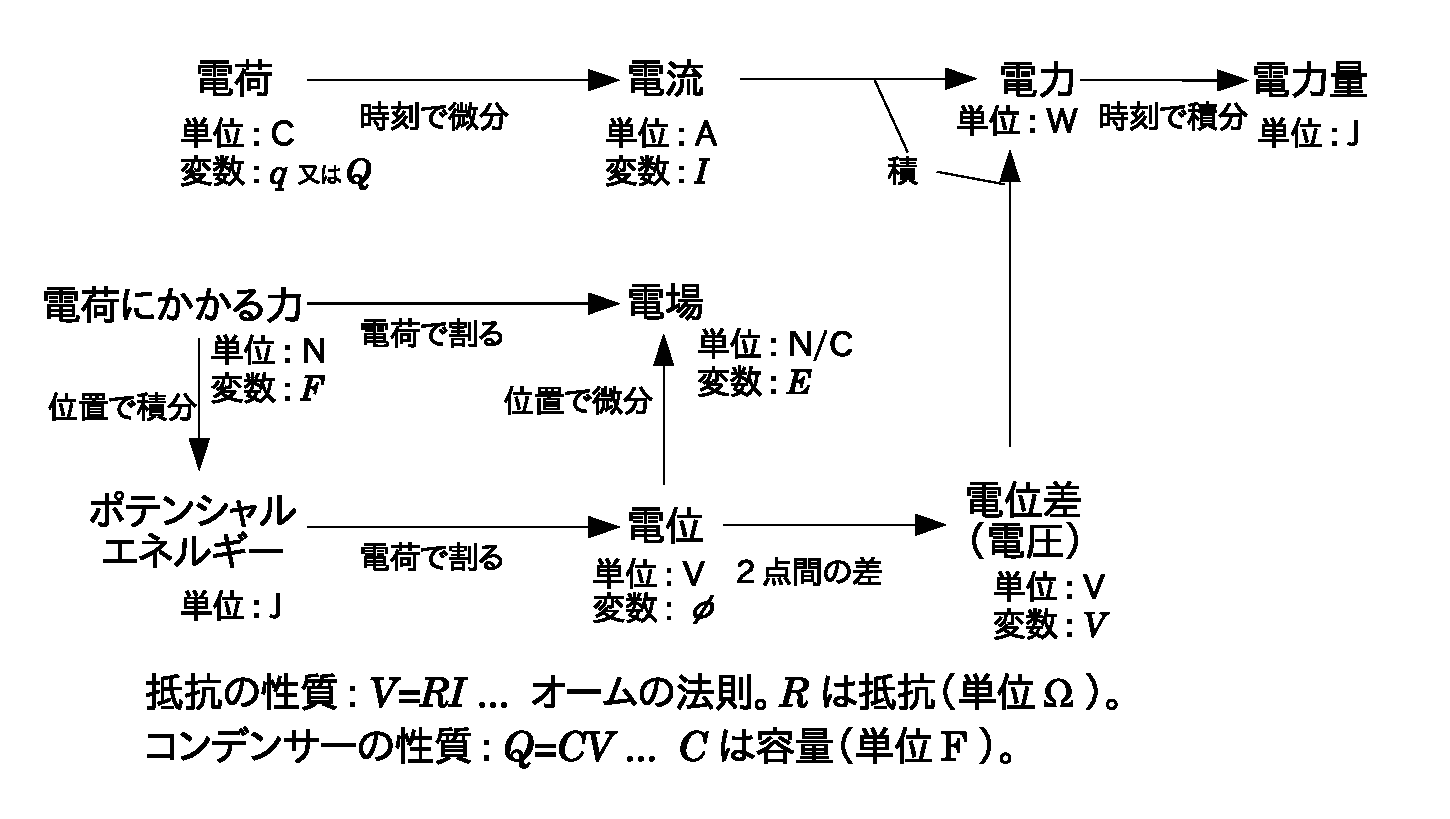
\includegraphics[width=8.5cm]{electronics.eps}
    \caption{電気に関する概念の関係図。斜字体と立体の区別に
注意せよ。斜字体は変数を, 立体は単位を表す。変数には, よく使われる
記号を示すが, 人によって例外もあることに注意せよ。単位の読み方
は, A: アンペア, C: クーロン, F: ファラド, J: ジュール, 
N: ニュートン, V: ボルト, W: ワット, $\Omega$: オーム}\label{fig:electronics}
\end{figure}

\begin{q}\label{eq:def_electricity} 電流・電力・電力量を, 
それぞれ簡潔に説明せよ。また, それぞれのSI単位を述べよ。
\end{q}\mv


\begin{q}\label{eq:battery_Ah} 電池の容量(電荷)を表すのに, A~h
という単位がよく使われる。ある自動車のバッテリー(8000円くらい)は, 
36A~hの容量だった。
\begin{enumerate}
\item このバッテリーが流すことのできる電荷の総量を求めよ。
\item このバッテリーができる仕事の総量を求めよ。ただし, この
バッテリーも含めて, 自動車のバッテリーはほとんどが電圧12~Vである。
\item ある車はこのバッテリーを積んでいる。この車のヘッドランプは
LEDであり, 片方が23~Wの消費電力である。左右両方のヘッドランプをつけっぱなし
にしたら, どのくらいの時間でバッテリーは空っぽになるか?
\end{enumerate}
\end{q}
\hv

\begin{exq} 昔は水田に水を入れるのに, 足踏み水車というものを使った。足踏み水車を使って, 
灌漑水路から水田(面積1~a)に水を入れようと思う。灌漑水路の水面と水田の
間には畦があり, 畦は水路水面よりも50~cm高い。この水田に, 水深5~cmになるまで水を
5時間で汲み上げる場合の仕事率を求めよ。\end{exq}
%1.4W

\begin{exq} 頂角60度の円錐があり、そこに質量100~gの円形の鎖がかぶさっている。
この鎖にかかる張力の大きさを求めよ。ただし円錐表面と鎖の間には摩擦は無い(つるつるしている)
とする。重力加速度は$g$=9.8~m~s$^{-2}$とする。\end{exq}


\section{解答}
% 
\noindent{\textbf{答}}\ref{q:def_work}
\begin{enumerate}
\item 力と, その力が働く点が力と同じ向きに動いた距離との, 積。
\item J = N~m=kg~m$^2$~s$^{-2}$。
\item 力がつりあっている系では, 仮想的な微小変位に伴って外力のなす仕事の総和は0である。
\end{enumerate}
\vspace{0.2cm}

% 
\noindent{\textbf{答}}\ref{q:teko}
\begin{enumerate}
\item 略(ヒント: 直角三角形の高さを三角関数で表す)。
\item 物体1について, 重力は鉛直下向きで$m_1g$である。その重力が働く
点である物体1の, 重力方向(鉛直下向き)への変位\footnote{位置の変化量
のことを変位(displacement)という。}は$h_1$であり, それは前問より$l_1\sin\theta$
である。従って, 重力が物体1にした仕事は
\begin{eqnarray}m_1gh_1=m_1gl_1\sin\theta\end{eqnarray}

物体2については, 重力は鉛直下向きで$m_2g$である。物体2の重力の方向
(鉛直下向き)への変位は$-h_2$である(マイナスがつくのは, 重力とは逆向きだから)。
それは前問より$-l_2\sin\theta$
である。従って, 重力が物体2にした仕事は
\begin{eqnarray}-m_2gh_2=-m_2gl_2\sin\theta\end{eqnarray}
\item 仮想仕事の原理より, 前問の2つの仕事の和は0だから, 
\begin{eqnarray}m_1gl_1\sin\theta-m_2gl_2\sin\theta=0\end{eqnarray}
従って, 
\begin{eqnarray}m_1l_1=m_2l_2\end{eqnarray}
\end{enumerate}
\vspace{0.2cm}

%
\noindent{\textbf{答}}\ref{q:jack}
\begin{enumerate}
\item ハンドルをまわす距離は$2\pi r$。ハンドルを回す力は, ハンドルの移動(回転)の
方向と常に一致しており, その大きさは$F$。したがって, ハンドルを1回転させるときに回す手がなす仕事は, 
$2\pi r F$。
\item ハンドルが1回転するときに, 上載物は$\Delta y$だけ持ち上がる。このとき, 上載物にかかる
重力は, 下向き(上載物の移動とは逆方向)に$mg$の大きさでかかるから, 重力のなす仕事は, 
$-mg\Delta y$となる。
\item ハンドルが1回転することを微小な変位であるとみなせば, 仮想仕事の原理より, 
ハンドルを回す手がなす仕事と重力がなす仕事の和は0である。従って与式が成り立つ。
\item 前小問の式を$F=$のように変形すればよい。
\item 前小問の式に各数値を代入して, 23 N。これは約2~kgの物体にかかる重力, つまり, 
2リットル入りのペットボトルを直接持ち上げる程度の力である。ジャッキを使えば, 
それで1000~kgの上載物を持ち上げることができるのだ。
\end{enumerate}

% 
\noindent{\textbf{答}}\ref{q:energy}
仕事が形を変えた量, もしくは仕事に形を変えることができる量。
\vspace{0.2cm}

% 
\noindent{\textbf{答}}\ref{q:spring_work}
仕事の定義\eref{eq:work2}で$F(x)=-kx$とすれば, 
\begin{eqnarray}W=\int_{x_0}^{x_1}(-kx)\,dx=-\frac{1}{2}k(x_1^2-x_0^2)\end{eqnarray}
\vspace{0.2cm}

% 
\noindent{\textbf{答}}\ref{q:gas_work} 
\begin{enumerate}
\item シリンダーの内部は, 底面積$A$, 高さ$h$の筒形の空間である。従ってその体積は$V=Ah$。
\item 気体は圧力$P$でピストンを押し上げようとする。一般に, 一定の圧力がかかる面には, 
圧力かける面積という大きさの力がかかる。従って, この場合は気体はピストンを$PA$という力で
押し上げようとする。いま, 座標軸を鉛直上向きにとっているので, 上向きが正。従って, $F_1=PA$。
\item ピストンは静止しているので, ピストンにかかる力はつりあっていなければならない。
従って$F_1$を打ち消す力が外から働いているはずである。従って外力は$F_2=-F_1=-PA$。
\item ピストンの移動がゆっくり(つまりほとんど静止しているということ)なので, 
力のつりあいは維持されると考えてよい。外力がなす仕事$dW$は, 力$F_2$と変位$dh$の積である。
従って, 
\begin{eqnarray}dW=F_2\,dh=-PA\,dh\end{eqnarray}
\item 変化前の気体の体積は$V=Ah$, 変化後の気体の体積は$V+dV=A(h+dh)$である。これらの式
より, $dV=A\,dh$を得る。
\item 略。
\item 略。(\eref{eq:gas_work5}を積分すればよい。)
\item 状態方程式より, $P=nRT/V$。これを前小問の結果に代入すれば与式を得る。
\item 温度一定なので, 前小問の式より, 
\begin{eqnarray}
W&=&-nRT\int_{V_1}^{V_2}\frac{dV}{V}=-nRT\Bigl[\ln|V|\Bigr]_{V_1}^{V_2}\nonumber\\
&=&-nRT\ln \frac{V_2}{V_1}=nRT\ln \frac{V_1}{V_2}
\end{eqnarray}
注: 体積$V_1, V_2$はいずれも正なので, 対数の中の絶対値記号は結局は不要になる。
\item $n=1\,$mol, $R=8.31$ J~mol$^{-1}$ K$^{-1}$, $T=273$ K, $V_1/V_2=2$, $\ln 2=\log_e 2\fallingdotseq0.693$
を前小問に代入し, $W=1570$ J。(有効数字3桁)
\end{enumerate}
\vspace{0.2cm}

% 
\noindent{\textbf{答}}\ref{q:def_potential}
ある基準点から任意の位置$x$まで物体を運ぶときの仕事
を$W(x)$とするとき, $U(x)=-W(x)$で定義される関数$U(x)$を
ポテンシャルエネルギーという。
\vspace{0.2cm}

% 
\noindent{\textbf{答}}\ref{q:potential_spring}
\eref{eq:spring_work}で, $x_0=0$, $x_1=x$とおきなおせば, 
\begin{eqnarray}
U(x)=-W(x)=\frac{1}{2}kx^2
\end{eqnarray}
\begin{figure}[h]
    \centering
    \includegraphics[width=6cm]{stringPE.eps}
    \caption{バネのポテンシャルエネルギー}\label{fig:stringPE}
\end{figure}
グラフは図\ref{fig:stringPE}のようになる。

% 
\noindent{\textbf{答}}\ref{q:potential_gravity}
\eref{eq:work_gravity}で, $R_0=\infty$, $R_1=R$とおきなおせば, 
\begin{eqnarray}
U(R)=-W(R)=-\frac{GMm}{R}
\end{eqnarray}
\begin{figure}[h]
    \centering
    \includegraphics[width=6cm]{gravityPE.eps}
    \caption{万有引力のポテンシャルエネルギー}\label{fig:gravityPE}
\end{figure}
グラフは図\ref{fig:gravityPE}のようになる。

\noindent{\textbf{答}}\ref{q:potential_etc}
\begin{enumerate}
\item \eref{eq:potential_g}において, $m=2$~kg, $g=9.8$~m~s$^{-2}$, $h=10$~mとすれば, 
$U=196\,\,\text{J}\fallingdotseq 200$ J
\item 問\ref{q:YoungModulus}(3)より, バネ定数$k$は, $k=6.2\times10^4$~kg s$^{-2}$。
また, $x=0.001$~mとして, これらを\eref{eq:potential_spring}に代入すれば, $U=0.031$ J。
\item 地球の質量を$M$, 月の質量を$m$, 地球と月の距離を$x$とすれば, 
\begin{eqnarray*}
G&=&6.7\times10^{-11}\,\text{ m}^3\,\,\text{kg}^{-1}\,\,\text{s}^{-2}\\
M&=&6.0\times10^{24}\,\text{ kg}\\
m&=&7.3\times10^{22}\,\text{ kg}\\
x&=&4.0\times10^{8}\,\text{ m}
\end{eqnarray*}
これらを\eref{eq:potential_gravity}に代入して, $U=-7.3\times10^{28}$ J。
(ただし無限遠を基準点とする。)
\end{enumerate}
\mv

% 傾斜角$\theta$の滑らかな斜面に沿って, 質量$m$の物体を, 斜距離$L$だけ運びあげた。
\noindent{\textbf{答}}\ref{q:slope_lift_energy1}
物体にかかる重力を, 斜面に垂直な方向と, 斜面に平行な方向に分解して考える。
前者は斜面から受ける垂直抗力と釣り合って打ち消しあう。後者は
\begin{eqnarray}mg\sin\theta\end{eqnarray}
となる($\theta$は傾斜角)。誰かがこれと等しい大きさの力を斜面に平行で上向きに
かけることで物体が斜距離$L$だけ移動する。そのとき「誰か」が行った仕事は, 
\begin{eqnarray}mgL\sin\theta\end{eqnarray}
となる。これはポテンシャルエネルギーの変化にも等しい。\mv


% 保存力とは何か? 
\noindent{\textbf{答}}\ref{q:conservative_force}
保存力とは, 物体をある位置から別の位置に運ぶときに
その力がなす仕事が, 移動の経路によらずに一定である, というような力である。\mv


% 摩擦力が保存力でないことを証明しよう。
\noindent{\textbf{答}}\ref{q:friction_non_conservative}
\begin{enumerate}
\item 物体を位置$x_0$から位置$x_1$に運んで位置$x_0$に戻す, という
移動も, 物体を位置$x_0$に置いたまま動かさない, というのも, ともに, 
「物体を位置$x_0$から位置$x_0$に移動する」経路である。前者の
仕事は$W_{01}+W_{10}$であり, 後者の仕事は0である(移動距離が無いから)。
従って, もし力が保存力なら, $W_{01}+W_{10}=0$である。
\item 動摩擦力の大きさを$F_{\text m}$とし, $x_0$と$x_1$の間の距離を$X$とすると, 
$W_{01}=-F_{\text m}X$である。ここでマイナスがつくのは, 力の向きが移動方向と
逆だからである。同様に, $W_{10}=-F_{\text m}X$である。従って, 
$W_{01}+W_{10}=-2F_{\text m}X$
となり, 前小問の式は成り立たない。従って摩擦力は保存力でない(背理法)。
\end{enumerate}
\mv

% 
\noindent{\textbf{答}}\ref{q:slope_lift_energy2}
問\ref{q:slope_lift_energy1}とほぼ同様だが, この場合, 物体には, 
斜面平行・下向きに, $\mu'mg\cos\theta$という摩擦力もかかる。そのぶん
「誰か」はがんばらねばならない。結果的に, 「誰か」が斜面に平行で上向きに
かける力は, 
\begin{eqnarray}mg\sin\theta+\mu'mg\cos\theta\end{eqnarray}
となる。
物体は斜距離$L$だけ移動するので, 「誰か」が行った仕事は, 
\begin{eqnarray}mgL\sin\theta+\mu'mgL\cos\theta\end{eqnarray}
となる。ところが, 摩擦力は保存力ではないので, ポテンシャルエネルギーの増減には
関与しない。従って, ポテンシャルエネルギーの増加は, $mgL\sin\theta$。\mv

\noindent{\textbf{答}}\ref{q:work_rate}
\eref{eq:work_rate_lift}に, $m=2.0$~kg, $g=9.8$~m~s$^{-2}$, $v=3.0$~m~s$^{-1}$を代入すると, 
有効数字2桁で$P= 59$ W。
\mv

%
\noindent{\textbf{答}}\ref{q:watt_hour}
1 W h = 1 J s$^{-1} \times 3600$ s=3600 J
\mv


\noindent{\textbf{答}}\ref{q:potential_Coulomb}
原点に電荷$Q$を固定し, $x$軸上に電荷$q$を動かす。位置$x$に電荷$q$があるとき($0<x$とする), 
それに働く力$F$は, \eref{eq:coulomb}より, 
\begin{eqnarray}
F=\frac{k\,Q\,q}{x^2}
\end{eqnarray}
である。無限遠から位置$x$まで電荷$q$を動かすときに, この力がなす仕事は, 
\begin{eqnarray}
W=\int_{\infty}^{x}F\,dx=\int_{\infty}^{x}\frac{k\,Q\,q}{x^2}\,dx
=\Bigl[-\frac{k\,Q\,q}{x}\Bigr]_{\infty}^{x}=-\frac{k\,Q\,q}{x}\nonumber\\\label{eq:potential_Coulomb00}
\end{eqnarray}
となる。\eref{eq:potential}より, 
\begin{eqnarray}
U(x)=-W=\frac{k\,Q\,q}{x}
\end{eqnarray}
となる(証明終わり)。\mv

{\small 注: \eref{eq:potential_Coulomb00}で, 積分変数$x$(つまり$dx$の$x$)と, 
積分区間の上端の$x$(つまり$\int_{\infty}^x$の$x$)が「かぶっている」が, 
これは別物と解釈する。すなわち積分変数$x$は, ほんとうは$X$とか$s$とか, 
何か適当に$x$以外の記号で置くのが数学的には正しいところだが, それは
めんどくさいしわかりにくくなるので, 横着して$x$のままにしておくのだ。このような
書き方は物理学でよく出てくる。\mv}

\noindent{\textbf{答}}\ref{q:potential_Coulomb2} 
\begin{enumerate}
\item \eref{eq:potential_Coulomb}を位置$x$における電荷$q$で割ればよい。
\begin{eqnarray}
\frac{U(x)}{q}=\frac{k\,Q}{x}\label{eq:voltage_Coulomb}
\end{eqnarray}
\item $x=0.529\times10^{-10}$~mとする。陽子の電荷は電荷素量なので
$Q=1.602\times10^{-19}$~C。また, \eref{eq:coulomb}より, 
$k=8.987\times 10^{9}$ N~m$^2$ C$^{-2}$。
これらを\eref{eq:voltage_Coulomb}に
代入すると, 27.2~V。
\end{enumerate}

\noindent{\textbf{答}}\ref{q:potential_Volt} 
\begin{enumerate}
\item 単位電荷あたりのポテンシャルエネルギー
\item 空間の2つの点の間を仮想的に荷電粒子を移動させるとき, 
かかる仕事を電荷で割ったもの。多くの場合, 2点間の電位の差(電位差)。
\item J~C$^{-1}$, 言い換えると, V。
\item 0.6~J
\item 電子の電荷は$-1.602\times10^{-19}$ Cなので, それが1~Vの電位にあると, 
$-1.602\times10^{-19}$ J。
\end{enumerate}
\mv


\noindent{\textbf{答}}\ref{q:radiation_eV}
\begin{enumerate}
\item $m_{\text{He}}=4$~g$/(6.0\times10^{23})$=...=6.7$\times10^{-27}$~kg。
\item $\alpha$線のエネルギーを$E$, 速さを$v$とすると, $\frac{1}{2}m_{\text{He}}v^2=E$。
従って, $v=\sqrt{2E/m_{\text{He}}}=...=1.6\times10^7$~m~s$^{-1}$。
\item $\beta$線のエネルギーを$E$, 速さを$v$とすると, 上と同様に, 
従って, $v=\sqrt{2E/m_{\text{e}}}=...=4.2\times10^8$~m~s$^{-1}$。
\end{enumerate}
注: eVをJに直して計算しないと, 正しい答にはならない。単位を埋め込んで計算すれば, 
それに気がつくはず!
\mv

%\noindent{\textbf{答}}\ref{eq:def_electricity} 略。
%\mv

\noindent{\textbf{答}}\ref{eq:battery_Ah} 
\begin{enumerate}
\item 36~A~h=36~(C/s)$\times$3600~s=130000~C。
\item 12~V$\times$36~A~h=$12\times36\times3600$~V~A~s=$1.6\times10^6$~J。
\item 左右両方で46~W。12~Vの電圧では, 46~W/(12~V) =3.8~Aの電流が
流れる。36~A~h/(3.8~A) =9.4~h。およそ9時間で空になる。これがLEDでなく, 
普通のハロゲンランプなら, もっと短い時間(数時間)で空になってしまう。
\end{enumerate}


\begin{faq}{\small\textgt{本当なのかなーって疑いたくなる値が答えだったり, 物理ってなんなんだー}
... 皆さんの既成概念を壊すために, そういうのを狙って問題を作ってます。}\end{faq}\mv

\begin{faq}{\small\textgt{代入する値がほしいです。}
 ... そのうち, 文字(変数)だけの答えにも慣れますよ。そっちのほうが, 
いろんな量どうしの関係がわかりやすい。}\end{faq}\mv

\begin{faq}{\small\textgt{「示せ」という問題は文も必要ですか? 言葉での説明が苦手です。}
 ... 言葉の定義をしっかり把握してください。その上で, まずは自分自身で納得できる説明を探すことが重要。}\end{faq}\mv

\begin{faq}{\small\textgt{なんとなくわかるけど, 問題解くときにわけわからなくなります。}
... だから問題演習は大事。しっかり考えて, わからなければ解答を読んで, また考えて下さい。}\end{faq}\mv

